\begin{figure}[ht]
\begin{center}
\begin{adjustbox}{width=0.7\textwidth}

\tikzset{every picture/.style={line width=0.75pt}} %set default line width to 0.75pt        

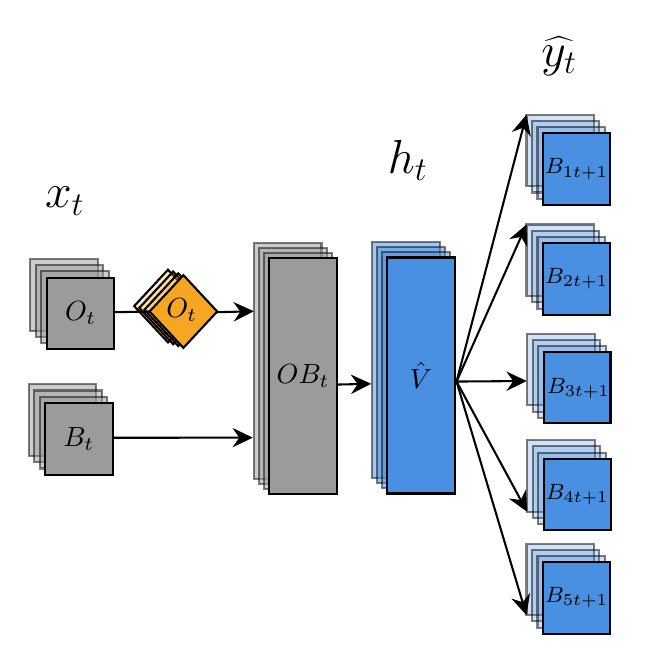
\begin{tikzpicture}[x=0.75pt,y=0.75pt,yscale=-1,xscale=1]
%uncomment if require: \path (0,331); %set diagram left start at 0, and has height of 331

%Shape: Diamond [id:dp8512741780313259] 
\draw  [fill={rgb, 255:red, 245; green, 166; blue, 35 }  ,fill opacity=0.25 ] (257.97,138.57) -- (274.27,156.09) -- (257.97,173.6) -- (241.68,156.09) -- cycle ;
%Shape: Diamond [id:dp44131568061643844] 
\draw  [fill={rgb, 255:red, 245; green, 166; blue, 35 }  ,fill opacity=0.25 ] (260.45,139.45) -- (276.74,156.96) -- (260.45,174.48) -- (244.15,156.96) -- cycle ;
%Shape: Diamond [id:dp9944377463655836] 
\draw  [fill={rgb, 255:red, 245; green, 166; blue, 35 }  ,fill opacity=0.25 ] (262.92,140.32) -- (279.22,157.84) -- (262.92,175.35) -- (246.63,157.84) -- cycle ;
%Shape: Rectangle [id:dp3605470636117536] 
\draw  [color={rgb, 255:red, 0; green, 0; blue, 0 }  ,draw opacity=0.5 ][fill={rgb, 255:red, 74; green, 144; blue, 226 }  ,fill opacity=0.5 ] (356.1,125.3) -- (388.87,125.3) -- (388.87,239) -- (356.1,239) -- cycle ;
%Shape: Rectangle [id:dp7194333726509892] 
\draw  [color={rgb, 255:red, 0; green, 0; blue, 0 }  ,draw opacity=0.5 ][fill={rgb, 255:red, 74; green, 144; blue, 226 }  ,fill opacity=0.5 ] (358.57,127.76) -- (391.34,127.76) -- (391.34,241.46) -- (358.57,241.46) -- cycle ;
%Shape: Rectangle [id:dp3276084138933598] 
\draw  [color={rgb, 255:red, 0; green, 0; blue, 0 }  ,draw opacity=0.5 ][fill={rgb, 255:red, 74; green, 144; blue, 226 }  ,fill opacity=0.5 ] (361.05,130.22) -- (393.82,130.22) -- (393.82,243.92) -- (361.05,243.92) -- cycle ;
%Shape: Diamond [id:dp6965315978812838] 
\draw  [fill={rgb, 255:red, 245; green, 166; blue, 35 }  ,fill opacity=1 ] (265.4,141.2) -- (281.69,158.71) -- (265.4,176.23) -- (249.1,158.71) -- cycle ;
%Straight Lines [id:da5408632178702979] 
\draw    (281.5,159.05) -- (296.35,158.66) ;
\draw [shift={(299.35,158.58)}, rotate = 178.5] [fill={rgb, 255:red, 0; green, 0; blue, 0 }  ][line width=0.08]  [draw opacity=0] (9.82,-4.72) -- (0,0) -- (9.82,4.72) -- (6.52,0) -- cycle    ;
%Straight Lines [id:da38550305545794683] 
\draw [fill={rgb, 255:red, 155; green, 155; blue, 155 }  ,fill opacity=1 ]   (209.09,219.56) -- (295.82,219.48) ;
\draw [shift={(298.82,219.48)}, rotate = 179.95] [fill={rgb, 255:red, 0; green, 0; blue, 0 }  ][line width=0.08]  [draw opacity=0] (9.82,-4.72) -- (0,0) -- (9.82,4.72) -- (6.52,0) -- cycle    ;
%Shape: Rectangle [id:dp8586026364143547] 
\draw  [color={rgb, 255:red, 0; green, 0; blue, 0 }  ,draw opacity=0.5 ][fill={rgb, 255:red, 74; green, 144; blue, 226 }  ,fill opacity=0.25 ] (430.7,116.78) -- (463.2,116.78) -- (463.2,151.29) -- (430.7,151.29) -- cycle ;
%Shape: Rectangle [id:dp5271658440371366] 
\draw  [color={rgb, 255:red, 0; green, 0; blue, 0 }  ,draw opacity=0.5 ][fill={rgb, 255:red, 74; green, 144; blue, 226 }  ,fill opacity=0.25 ] (433.34,119.76) -- (465.84,119.76) -- (465.84,154.27) -- (433.34,154.27) -- cycle ;
%Shape: Rectangle [id:dp6121896210605144] 
\draw  [color={rgb, 255:red, 0; green, 0; blue, 0 }  ,draw opacity=0.5 ][fill={rgb, 255:red, 74; green, 144; blue, 226 }  ,fill opacity=0.25 ] (436,122.81) -- (468.51,122.81) -- (468.51,157.32) -- (436,157.32) -- cycle ;
%Shape: Rectangle [id:dp2571940122217342] 
\draw  [fill={rgb, 255:red, 74; green, 144; blue, 226 }  ,fill opacity=1 ] (438.61,125.75) -- (471.11,125.75) -- (471.11,160.25) -- (438.61,160.25) -- cycle ;
%Shape: Rectangle [id:dp04921858860159267] 
\draw  [color={rgb, 255:red, 0; green, 0; blue, 0 }  ,draw opacity=0.5 ][fill={rgb, 255:red, 74; green, 144; blue, 226 }  ,fill opacity=0.25 ] (431.03,169.45) -- (463.53,169.45) -- (463.53,203.95) -- (431.03,203.95) -- cycle ;
%Shape: Rectangle [id:dp5512084563866699] 
\draw  [color={rgb, 255:red, 0; green, 0; blue, 0 }  ,draw opacity=0.5 ][fill={rgb, 255:red, 74; green, 144; blue, 226 }  ,fill opacity=0.25 ] (433.67,172.43) -- (466.17,172.43) -- (466.17,206.93) -- (433.67,206.93) -- cycle ;
%Shape: Rectangle [id:dp948946889597384] 
\draw  [color={rgb, 255:red, 0; green, 0; blue, 0 }  ,draw opacity=0.5 ][fill={rgb, 255:red, 74; green, 144; blue, 226 }  ,fill opacity=0.25 ] (436.33,175.48) -- (468.84,175.48) -- (468.84,209.98) -- (436.33,209.98) -- cycle ;
%Shape: Rectangle [id:dp7446725750615967] 
\draw  [fill={rgb, 255:red, 74; green, 144; blue, 226 }  ,fill opacity=1 ] (438.95,178.41) -- (471.17,178.41) -- (471.17,212.61) -- (438.95,212.61) -- cycle ;
%Shape: Rectangle [id:dp2953756097578333] 
\draw  [color={rgb, 255:red, 0; green, 0; blue, 0 }  ,draw opacity=0.5 ][fill={rgb, 255:red, 74; green, 144; blue, 226 }  ,fill opacity=0.25 ] (430.7,270.5) -- (463.2,270.5) -- (463.2,305.01) -- (430.7,305.01) -- cycle ;
%Shape: Rectangle [id:dp8190984811103563] 
\draw  [color={rgb, 255:red, 0; green, 0; blue, 0 }  ,draw opacity=0.5 ][fill={rgb, 255:red, 74; green, 144; blue, 226 }  ,fill opacity=0.25 ] (433.34,273.48) -- (465.84,273.48) -- (465.84,307.99) -- (433.34,307.99) -- cycle ;
%Shape: Rectangle [id:dp1989563986467071] 
\draw  [color={rgb, 255:red, 0; green, 0; blue, 0 }  ,draw opacity=0.5 ][fill={rgb, 255:red, 74; green, 144; blue, 226 }  ,fill opacity=0.25 ] (436,276.53) -- (468.51,276.53) -- (468.51,311.04) -- (436,311.04) -- cycle ;
%Shape: Rectangle [id:dp1924397511107222] 
\draw  [fill={rgb, 255:red, 74; green, 144; blue, 226 }  ,fill opacity=1 ] (438.61,279.47) -- (471.11,279.47) -- (471.11,313.98) -- (438.61,313.98) -- cycle ;
%Shape: Rectangle [id:dp8187051960536611] 
\draw  [color={rgb, 255:red, 0; green, 0; blue, 0 }  ,draw opacity=0.5 ][fill={rgb, 255:red, 74; green, 144; blue, 226 }  ,fill opacity=0.25 ] (431.03,220.71) -- (463.53,220.71) -- (463.53,255.22) -- (431.03,255.22) -- cycle ;
%Shape: Rectangle [id:dp6023578581008111] 
\draw  [color={rgb, 255:red, 0; green, 0; blue, 0 }  ,draw opacity=0.5 ][fill={rgb, 255:red, 74; green, 144; blue, 226 }  ,fill opacity=0.25 ] (433.67,223.69) -- (466.17,223.69) -- (466.17,258.2) -- (433.67,258.2) -- cycle ;
%Shape: Rectangle [id:dp8798703561171738] 
\draw  [color={rgb, 255:red, 0; green, 0; blue, 0 }  ,draw opacity=0.5 ][fill={rgb, 255:red, 74; green, 144; blue, 226 }  ,fill opacity=0.25 ] (436.33,226.74) -- (468.84,226.74) -- (468.84,261.25) -- (436.33,261.25) -- cycle ;
%Shape: Rectangle [id:dp3283044450373016] 
\draw  [fill={rgb, 255:red, 74; green, 144; blue, 226 }  ,fill opacity=1 ] (438.94,229.68) -- (471.44,229.68) -- (471.44,264.19) -- (438.94,264.19) -- cycle ;
%Shape: Rectangle [id:dp15154204076473643] 
\draw  [color={rgb, 255:red, 0; green, 0; blue, 0 }  ,draw opacity=0.5 ][fill={rgb, 255:red, 155; green, 155; blue, 155 }  ,fill opacity=0.5 ] (190.87,193.8) -- (223.37,193.8) -- (223.37,228.31) -- (190.87,228.31) -- cycle ;
%Shape: Rectangle [id:dp9182207029607203] 
\draw  [color={rgb, 255:red, 0; green, 0; blue, 0 }  ,draw opacity=0.5 ][fill={rgb, 255:red, 155; green, 155; blue, 155 }  ,fill opacity=0.5 ] (193.51,196.78) -- (226.01,196.78) -- (226.01,231.28) -- (193.51,231.28) -- cycle ;
%Shape: Rectangle [id:dp7698171692832448] 
\draw  [color={rgb, 255:red, 0; green, 0; blue, 0 }  ,draw opacity=0.5 ][fill={rgb, 255:red, 155; green, 155; blue, 155 }  ,fill opacity=0.5 ] (196.17,199.83) -- (228.68,199.83) -- (228.68,234.34) -- (196.17,234.34) -- cycle ;
%Shape: Rectangle [id:dp3865383455450443] 
\draw  [fill={rgb, 255:red, 155; green, 155; blue, 155 }  ,fill opacity=1 ] (198.78,202.77) -- (231.28,202.77) -- (231.28,237.27) -- (198.78,237.27) -- cycle ;
%Shape: Rectangle [id:dp23172130161456372] 
\draw  [fill={rgb, 255:red, 74; green, 144; blue, 226 }  ,fill opacity=1 ] (363.52,132.67) -- (396.29,132.67) -- (396.29,246.37) -- (363.52,246.37) -- cycle ;
%Shape: Rectangle [id:dp18125329077839125] 
\draw  [color={rgb, 255:red, 0; green, 0; blue, 0 }  ,draw opacity=0.5 ][fill={rgb, 255:red, 74; green, 144; blue, 226 }  ,fill opacity=0.25 ] (430.7,63.87) -- (463.2,63.87) -- (463.2,98.37) -- (430.7,98.37) -- cycle ;
%Shape: Rectangle [id:dp3729389269249752] 
\draw  [color={rgb, 255:red, 0; green, 0; blue, 0 }  ,draw opacity=0.5 ][fill={rgb, 255:red, 74; green, 144; blue, 226 }  ,fill opacity=0.25 ] (433.34,66.84) -- (465.84,66.84) -- (465.84,101.35) -- (433.34,101.35) -- cycle ;
%Shape: Rectangle [id:dp8889532693849542] 
\draw  [color={rgb, 255:red, 0; green, 0; blue, 0 }  ,draw opacity=0.5 ][fill={rgb, 255:red, 74; green, 144; blue, 226 }  ,fill opacity=0.25 ] (436,69.9) -- (468.51,69.9) -- (468.51,104.4) -- (436,104.4) -- cycle ;
%Shape: Rectangle [id:dp22768677359456946] 
\draw  [fill={rgb, 255:red, 74; green, 144; blue, 226 }  ,fill opacity=1 ] (438.61,72.83) -- (471.11,72.83) -- (471.11,107.34) -- (438.61,107.34) -- cycle ;
%Straight Lines [id:da6521632540749734] 
\draw    (397,192.45) -- (429.94,66.77) ;
\draw [shift={(430.7,63.87)}, rotate = 104.68] [fill={rgb, 255:red, 0; green, 0; blue, 0 }  ][line width=0.08]  [draw opacity=0] (9.82,-4.72) -- (0,0) -- (9.82,4.72) -- (6.52,0) -- cycle    ;
%Straight Lines [id:da4098284445759105] 
\draw    (397,192.45) -- (429.48,119.52) ;
\draw [shift={(430.7,116.78)}, rotate = 114] [fill={rgb, 255:red, 0; green, 0; blue, 0 }  ][line width=0.08]  [draw opacity=0] (9.82,-4.72) -- (0,0) -- (9.82,4.72) -- (6.52,0) -- cycle    ;
%Straight Lines [id:da6632019398295455] 
\draw    (397,192.45) -- (427.8,192.22) ;
\draw [shift={(430.8,192.2)}, rotate = 179.57] [fill={rgb, 255:red, 0; green, 0; blue, 0 }  ][line width=0.08]  [draw opacity=0] (9.82,-4.72) -- (0,0) -- (9.82,4.72) -- (6.52,0) -- cycle    ;
%Straight Lines [id:da3742350341861914] 
\draw    (397,192.45) -- (429.6,252.58) ;
\draw [shift={(431.03,255.22)}, rotate = 241.54] [fill={rgb, 255:red, 0; green, 0; blue, 0 }  ][line width=0.08]  [draw opacity=0] (9.82,-4.72) -- (0,0) -- (9.82,4.72) -- (6.52,0) -- cycle    ;
%Straight Lines [id:da8736791937763184] 
\draw    (397,192.45) -- (429.84,302.14) ;
\draw [shift={(430.7,305.01)}, rotate = 253.33] [fill={rgb, 255:red, 0; green, 0; blue, 0 }  ][line width=0.08]  [draw opacity=0] (9.82,-4.72) -- (0,0) -- (9.82,4.72) -- (6.52,0) -- cycle    ;
%Shape: Rectangle [id:dp20286680685222525] 
\draw  [color={rgb, 255:red, 0; green, 0; blue, 0 }  ,draw opacity=0.5 ][fill={rgb, 255:red, 155; green, 155; blue, 155 }  ,fill opacity=0.5 ] (191.69,133.37) -- (224.2,133.37) -- (224.2,167.88) -- (191.69,167.88) -- cycle ;
%Shape: Rectangle [id:dp3612691236911778] 
\draw  [color={rgb, 255:red, 0; green, 0; blue, 0 }  ,draw opacity=0.5 ][fill={rgb, 255:red, 155; green, 155; blue, 155 }  ,fill opacity=0.5 ] (194.33,136.35) -- (226.84,136.35) -- (226.84,170.85) -- (194.33,170.85) -- cycle ;
%Shape: Rectangle [id:dp27994822217022974] 
\draw  [color={rgb, 255:red, 0; green, 0; blue, 0 }  ,draw opacity=0.5 ][fill={rgb, 255:red, 155; green, 155; blue, 155 }  ,fill opacity=0.5 ] (197,139.4) -- (229.5,139.4) -- (229.5,173.91) -- (197,173.91) -- cycle ;
%Shape: Rectangle [id:dp8551279256791401] 
\draw  [fill={rgb, 255:red, 155; green, 155; blue, 155 }  ,fill opacity=1 ] (199.6,142.34) -- (232.11,142.34) -- (232.11,176.84) -- (199.6,176.84) -- cycle ;
%Straight Lines [id:da9406188534668796] 
\draw    (232,159.05) -- (249.1,158.71) ;
%Shape: Rectangle [id:dp7419370874435655] 
\draw  [color={rgb, 255:red, 0; green, 0; blue, 0 }  ,draw opacity=0.5 ][fill={rgb, 255:red, 155; green, 155; blue, 155 }  ,fill opacity=0.5 ] (299.41,125.73) -- (331.92,125.73) -- (331.92,239.47) -- (299.41,239.47) -- cycle ;
%Shape: Rectangle [id:dp5764885214996254] 
\draw  [color={rgb, 255:red, 0; green, 0; blue, 0 }  ,draw opacity=0.5 ][fill={rgb, 255:red, 155; green, 155; blue, 155 }  ,fill opacity=0.5 ] (301.86,128.19) -- (334.38,128.19) -- (334.38,241.93) -- (301.86,241.93) -- cycle ;
%Shape: Rectangle [id:dp2742309190946596] 
\draw  [color={rgb, 255:red, 0; green, 0; blue, 0 }  ,draw opacity=0.5 ][fill={rgb, 255:red, 155; green, 155; blue, 155 }  ,fill opacity=0.5 ] (304.32,130.65) -- (336.84,130.65) -- (336.84,244.38) -- (304.32,244.38) -- cycle ;
%Straight Lines [id:da9649197155823988] 
\draw [fill={rgb, 255:red, 155; green, 155; blue, 155 }  ,fill opacity=1 ]   (331.42,194.09) -- (352.87,193.6) ;
\draw [shift={(355.87,193.53)}, rotate = 178.7] [fill={rgb, 255:red, 0; green, 0; blue, 0 }  ][line width=0.08]  [draw opacity=0] (9.82,-4.72) -- (0,0) -- (9.82,4.72) -- (6.52,0) -- cycle    ;
%Shape: Rectangle [id:dp877224255393874] 
\draw  [fill={rgb, 255:red, 155; green, 155; blue, 155 }  ,fill opacity=1 ] (306.77,133.11) -- (339.29,133.11) -- (339.29,246.84) -- (306.77,246.84) -- cycle ;

% Text Node
\draw (454.86,143) node  [font=\footnotesize]  {$B_{2t+1}$};
% Text Node
\draw (455.74,195.67) node  [font=\footnotesize]  {$B_{3t+1}$};
% Text Node
\draw (455.19,246.93) node  [font=\footnotesize]  {$B_{4t+1}$};
% Text Node
\draw (454.86,296.72) node  [font=\footnotesize]  {$B_{5t+1}$};
% Text Node
\draw (215.03,220.02) node  [font=\normalsize]  {$B_{t}$};
% Text Node
\draw (264.57,157.84) node  [font=\normalsize]  {$O_{t}$};
% Text Node
\draw (446.54,35.73) node  [font=\LARGE]  {$\widehat{y_{t}}$};
% Text Node
\draw (208.33,105.54) node  [font=\LARGE]  {$x_{t}$};
% Text Node
\draw (379.91,189.52) node  [font=\normalsize]  {$\hat{V}$};
% Text Node
\draw (454.86,90.09) node  [font=\footnotesize]  {$B_{1t+1}$};
% Text Node
\draw (215.86,159.59) node  [font=\normalsize]  {$O_{t}$};
% Text Node
\draw (323.03,189.98) node  [font=\normalsize]  {$OB_{t}$};
% Text Node
\draw (373.54,85.73) node  [font=\LARGE]  {$h_{t}$};


\end{tikzpicture}

\end{adjustbox}
\end{center}
\caption[\textbf{The time distributed multi-layer perceptron architecture}]{Blue and orange shapes represent respectively feedforward and embedding operations. Gray shapes indicate operations with no learnable parameters, such as tensor instantiation and concatenation. Stacked, transparent colouring indicates tensors with a sequential structure. Straight arrows refer to the presence of feed-forward information flow. All the feedforward operations are time distributed.}
\label{fig: mlp_2}
\end{figure}